%%%%%%%%%%%%%%%%%%%%%%%%%%%%%%%%%%%%%%%%%%%%%%%%%%%%%%%%%%%%%%%%%%%%%%
\begin{frame}[fragile]\frametitle{}
\begin{center}
{\Large Problems and Solutions from LeetCode}
\end{center}

	{\tiny (Ref :  https://www.youtube.com/watch?v=sUicrnHwA0s\&list=PLiC1doDIe9rDFw1v-pPMBYvD6k1ZotNRO , https://www.youtube.com/c/NeetCode/videos)}

\end{frame}

%%%%%%%%%%%%%%%%%%%%%%%%%%%%%%%%%%%%%%%%%%%%%%%%%%%%%%%%%%%%%%%%%%%%%%
\begin{frame}[fragile]\frametitle{1. Two Sum (Easy)}

	\begin{itemize}
	\item Given an array of integers, return indices of the two numbers such that they add up to a specific target
	\item \lstinline|nums =  [2,7,11,15], target = 9, as nums[0] + nums[1] = 2 + 7 = 9, return [0,1]|
	\end{itemize}
	
	\begin{columns}[T]
		\column{0.455\linewidth}
		\begin{lstlisting}[basicstyle=\scriptsize]
# Brute force ie two for loops, so O(n^2)
def two_sum_brute(nums, target):
		for i in range(len(nums) - 1):
				for j in range(i + 1, len(nums)):
						if nums[i] + nums[j] == target:
								return [i, j]
		return [-1, -1]		
		\end{lstlisting}
		\column{0.455\linewidth}
		\begin{lstlisting}[basicstyle=\scriptsize]
# Loop once, dictionary based, so O(n)
def two_sum_dict(nums, target):
		seen = {}
		for i, num in enumerate(nums):
				if target - num in seen:
						return [seen[target - num], i]
				elif num not in seen:
						seen[num] = i
		return [-1, -1]	
				\end{lstlisting}		
	\end{columns}
	
	
\end{frame}

%%%%%%%%%%%%%%%%%%%%%%%%%%%%%%%%%%%%%%%%%%%%%%%%%%%%%%%%%%%%%%%%%%%%%%
\begin{frame}[fragile]\frametitle{4. Median of Two Sorted Arrays (Hard)}

	\begin{itemize}
	\item aaa
	\item Example \lstinline|aaa|
	\end{itemize}
	
	\begin{columns}[T]
		\column{0.455\linewidth}
		\begin{lstlisting}[basicstyle=\scriptsize]
aaa
		\end{lstlisting}
		\column{0.455\linewidth}
		\begin{lstlisting}[basicstyle=\scriptsize]
aaa
				\end{lstlisting}		
	\end{columns}
	
	
\end{frame}

%%%%%%%%%%%%%%%%%%%%%%%%%%%%%%%%%%%%%%%%%%%%%%%%%%%%%%%%%%%%%%%%%%%%%%
\begin{frame}[fragile]\frametitle{2. Add Two Numbers}


	\begin{itemize}
	\item Given two linked lists representing 2 numbers, digits are stored in reverse order. Add both and return result as list
	\item \lstinline|(2->4->3) + (5->6->4), so numbers are 342 + 465 = 807, so result is (7->0->8)|
	\end{itemize}
	
	\begin{columns}[T]
		\column{0.455\linewidth}
		\begin{lstlisting}[basicstyle=\scriptsize]
# Definition of singly-linked list
class ListNode:
    def __init__(self, val=0, next=None):
        self.val = val
        self.next = next
				
# position wise addition, and carry forward
def addTwoNumbers(l1, l2):
    added = ListNode(val=(l1.val + l2.val) % 10)
    carry_over = (l1.val + l2.val) // 10
    current_node = added
    while (l1.next and l2.next):
        l1 = l1.next
        l2 = l2.next
				current_sum = carry_over + l1.val + l2.val
        current_node.next = ListNode(val=current_sum % 10)
        carry_over = current_sum // 10
        current_node = current_node.next				
		\end{lstlisting}
		\column{0.455\linewidth}
		\begin{lstlisting}[basicstyle=\scriptsize]
    while(l1.next):
        l1 = l1.next
				current_sum = carry_over + l1.val 
        current_node.next = ListNode(val=current_sum % 10)
        carry_over = current_sum // 10
        current_node = current_node.next

    while(l2.next):
        l2 = l2.next
				current_sum = carry_over + l2.val
        current_node.next = ListNode(val=current_sum % 10)
        carry_over = current_sum // 10
        current_node = current_node.next

    if carry_over > 0:
        current_node.next = ListNode(val=1)
    return added
				\end{lstlisting}		
	\end{columns}
	
\end{frame}

%%%%%%%%%%%%%%%%%%%%%%%%%%%%%%%%%%%%%%%%%%%%%%%%%%%%%%%%%%%%%%%%%%%%%%
\begin{frame}[fragile]\frametitle{3. Longest Substring without repeating characters}


	\begin{itemize}
	\item Given a string find the length of the longest substring without repeating characters
	\item \lstinline|"abcabcbb" => 3 for "abc" ; "bbbbbbbbbb" => 1 for "b"|
	\end{itemize}
	
	\begin{columns}[T]
		\column{0.5\linewidth}
	\begin{itemize}
	\item Go on string letters one by one, store each with its index, till you find a duplicate 
	\item In ``abcabcbb'' you will go till 2nd `a', storing \lstinline|{'a'=0,'b'=1,'c'=2}| 
	\item Once duplicate is found, within the same substring, reset start of the next search at letter next to first duplicates ie 2nd 'b'
	\item Capture current substring length as current index which is 3 - index of the first conflict letter, ie 0, so length = 3
	\item Start search similarly from 2nd 'b'
	\end{itemize}
		\column{0.455\linewidth}
		\begin{lstlisting}[basicstyle=\scriptsize]
def lengthOfLongestSubstring(s):
    substring = dict()
    current_substring_start = 0
    current_substring_length = 0
    longest_substring_sofar = 0
    for i, letter in enumerate(s):
        if letter in substring and substring[letter] >= current_substring_start:
            current_substring_start = substring[letter] + 1
            current_substring_length = i - substring[letter]
            substring[letter] = i
        else:
            substring[letter] = i
            current_substring_length += 1
            if current_substring_length > longest_substring_sofar:
                longest_substring_sofar = current_substring_length
    return longest_substring_sofar
				\end{lstlisting}		
	\end{columns}
	
\end{frame}

%%%%%%%%%%%%%%%%%%%%%%%%%%%%%%%%%%%%%%%%%%%%%%%%%%%%%%%%%%%%%%%%%%%%%%
\begin{frame}[fragile]\frametitle{5. Longest Palindromic Substring}


	\begin{itemize}
	\item Given a string s, return longest palindromic substring in s
	\item \lstinline|"babad" => "bab", "aba"|
	\item Brute Force: e.g. ``abcbd''. Brute force could be to run 2 for loops, for different ranges, longest to shortest and check for palindrome, return first hit of the longest
	\item Better to find centers having palindrome around it, by expanding step by step. Store biggest so far. Take care of Odd and Even lengths. Find lengthier than current biggest.
	\end{itemize}
	


		\begin{lstlisting}[basicstyle=\scriptsize]
def is_palindrome(s):
    return s == s[::-1]
		
def longestPalindromicSubstring_bruteforce(s):
    for length in range(len(s), 0, -1):  # reverse length numbers
        for start_index in range(0, len(s) + 1 - length):  # different starting points
            current_substring = s[start_index:(start_index + length)]
            if is_palindrome(current_substring):
                return current_substring  # return right away because we are checking the longest first
		\end{lstlisting}		


\end{frame}

%%%%%%%%%%%%%%%%%%%%%%%%%%%%%%%%%%%%%%%%%%%%%%%%%%%%%%%%%%%%%%%%%%%%%%
\begin{frame}[fragile]\frametitle{5. Longest Palindromic Substring}

		\begin{lstlisting}[basicstyle=\scriptsize]
def longestPalindromicSubstring(s):
    biggest = s[0]
    step = len(biggest) // 2  # one side
    # odd case
    for center in range(1, len(s) - 1):
        bounds = [center - (1 + step), center + (1 + step)]  # both directions
        while (bounds[0] > -1) and (bounds[1] < len(s)):  # ends
            current_string = s[bounds[0]:bounds[1] + 1]
            if is_palindrome(current_string):
                biggest = current_string
                step = len(biggest) // 2  # find longer next
                bounds[0] -= 1  # make wider
                bounds[1] += 1
            else:
                break
    # even case
    for center in range(step, len(s) - step - 1):
        bounds = [center - step, center + (1 + step)]  # both directions
        while (bounds[0] > -1) and (bounds[1] < len(s)):  # ends
            current_string = s[bounds[0]:bounds[1] + 1]
            if is_palindrome(current_string):
                biggest = current_string
                step = len(biggest) // 2  # find longer next
                bounds[0] -= 1  # make wider
                bounds[1] += 1
            else:
                break
    return biggest
		\end{lstlisting}		

\end{frame}

%%%%%%%%%%%%%%%%%%%%%%%%%%%%%%%%%%%%%%%%%%%%%%%%%%%%%%%%%%%%%%%%%%%%%%
\begin{frame}[fragile]\frametitle{6. ZigZag Conversion}


	\begin{itemize}
	\item Write code that will take a string and make zig zag on given number of rows
\lstinline{"Paypal is hiring" ie "PAYPALISHIRING" => |/|/| like order}
	\item Output : ``PAHNAPLSIIGYIR''
	\item Dictionary based solution, each key is for a row value is list of letters in it.
	\item Go on increasing row counter till num, then decreasing till 1 and so on.
	\end{itemize}

		\begin{lstlisting}[basicstyle=\scriptsize]
def convert_zigzag(s, num):
    if num == 1:
        return s
    rows_dict = {row: "" for row in range(1, num + 1)}
    current_row_index = 1
    increment_row_index = True # False for down
    for c in s: # each letter:
        rows_dict[current_row_index] += c
        if (current_row_index == 1) or ((current_row_index < num) and increment_row_index):
            current_row_index += 1
            increment_row_index = True
        else:
            current_row_index -= 1
            increment_row_index = False
    converted_string = ""
    for row in range(1, num+1):
        converted_string += rows_dict[row]
    return converted_string		
				\end{lstlisting}		

	
\end{frame}

%%%%%%%%%%%%%%%%%%%%%%%%%%%%%%%%%%%%%%%%%%%%%%%%%%%%%%%%%%%%%%%%%%%%%%
\begin{frame}[fragile]\frametitle{9. Palindrome Number}


	\begin{itemize}
	\item Determine if given integer is palindrome, without converting integer to string. Example121 is, -121 is not
	\item Conversion solution : \lstinline{return (str(x) == str(x)[::-1])}
	\item If number is negative, return False directly, as "-" can not be on right end.
	\item Separate out digits then reverse, and check with original by equality
	\end{itemize}

		\begin{lstlisting}[basicstyle=\scriptsize]
def is_palindrome(x):
    if x < 0:
        return False
    reversed_num = 0
    decimal_step = 0
    while (x // (10 ** decimal_step) !=0):
        reversed_num = (reversed_num * 10) + (x // (10 ** decimal_step) % 10)
        decimal_step += 1

    return (x == reversed_num)
				\end{lstlisting}		

	
\end{frame}

%%%%%%%%%%%%%%%%%%%%%%%%%%%%%%%%%%%%%%%%%%%%%%%%%%%%%%%%%%%%%%%%%%%%%%
\begin{frame}[fragile]\frametitle{11. Container With Most Water}


	\begin{itemize}
	\item Build histogram of numbers. With two bars as sides, find which container has most water
	\item For \lstinline{ [1,8,6,2,5,4,8,3,7] = 49}, between first and last
	\item Height as well as wider separation is needed.
	\item Brute force will be to try all pairs and finding max.
	\item Start from both ends and move in from shorter side and check.
	\end{itemize}

		\begin{lstlisting}[basicstyle=\scriptsize]
def maxArea(height):
    start_index = 0
    end_index = len(height) - 1
    largest = 0
    while start_index != end_index:
        next_area = min(height[start_index],height[end_index]) * (end_index - start_index)
        if next_area > largest:
            largest = next_area
        if height[start_index] < height[end_index]:
            start_index += 1
        else:
            end_index -= 1
    return largest
				\end{lstlisting}		

	
\end{frame}

%%%%%%%%%%%%%%%%%%%%%%%%%%%%%%%%%%%%%%%%%%%%%%%%%%%%%%%%%%%%%%%%%%%%%%
\begin{frame}[fragile]\frametitle{13. Roman to Integer}

	\begin{columns}[T]
		\column{0.5\linewidth}
	\begin{itemize}
	\item Compute integer number from Roman numerals number string
	\item \lstinline{ "LVIII" = 58, "IV" = 4, "MCMXCIV" = 1994}
	\item Letters have values from bigger to smaller and they are added.
	\item But in some cases, where lower letter is before higher, then value has to be subtracted.
	\item Start from left, towards right.
	\end{itemize}
		\column{0.455\linewidth}
		\begin{lstlisting}[basicstyle=\scriptsize]
def romanToInteger(s):
    roman_table = {"I": 1,
                   "V": 5,
                   "X": 10,
                   "L": 50,
                   "C": 100,
                   "D": 500,
                   "M": 1000}
    num = 0
    last = "I"
    for numeral in s [::-1]:
        if roman_table[numeral] < roman_table[last]:
            num -= roman_table[numeral]
        else:
            num += roman_table[numeral]
        last = numeral
    return num
				\end{lstlisting}		

	\end{columns}
		
\end{frame}

%%%%%%%%%%%%%%%%%%%%%%%%%%%%%%%%%%%%%%%%%%%%%%%%%%%%%%%%%%%%%%%%%%%%%%
\begin{frame}[fragile]\frametitle{14. Longest Common Prefix}

	\begin{columns}[T]
		\column{0.5\linewidth}
	\begin{itemize}
	\item Find The Longest Common Prefix amongst given strings
	\item \lstinline{ ["flower", "flow", "flight"] => "fl"}
	\item Start with first word as prefix and then go on reducing it with common prefix.
	\end{itemize}
		\column{0.455\linewidth}
		\begin{lstlisting}[basicstyle=\scriptsize]
def longestCommonPrefix(strs):
    if len(strs) == 0:
        return ""
    if len(strs) == 1:
        return strs[0]
    prefix = strs[0]
    prefix_length = len(prefix)
    for s in strs[1:]:
        while prefix != s[0:prefix_length]:
            prefix = prefix[0:prefix_length-1]
            prefix_length -= 1
            if prefix_length == 0:
                return ""
    return prefix
				\end{lstlisting}		

	\end{columns}
		
\end{frame}

%%%%%%%%%%%%%%%%%%%%%%%%%%%%%%%%%%%%%%%%%%%%%%%%%%%%%%%%%%%%%%%%%%%%%%
\begin{frame}[fragile]\frametitle{15. 3 Sum}

	\begin{columns}[T]
		\column{0.5\linewidth}
	\begin{itemize}
	\item Given number of n integers, are there 3 elements, $a,b,c$ where $a+b+c = 0$.
	\item \lstinline{ [-1,0,1,2,-1,-4] => [[-1,-1,2],[-1,0,-1]]}
	\item Brute force is 3 for loops, to get all combinations, and check the sum
	\item Sort the array. Fix first number in a single for loop. Then find pair that makes sum 0.
	\item For the pair, fix 'start' and 'end' at two extremes. If $sum > 0$, move 'end' towards left. If $sum < 0$, move 'start' towards right.
	\end{itemize}
		\column{0.455\linewidth}
		\begin{lstlisting}[basicstyle=\scriptsize]
def threeSum(nums):
    if len(nums) < 3:
        return []
    nums = sorted(nums)
    triplets = []
    for i in range(0,len(nums)-2):
        start = i +1
        end = len(nums) - 1
        while start < end:
            s = nums[i] + nums[start] + nums[end]
            if s == 0:
                triplets.append((nums[i],nums[start],nums[end]))
                start += 1
            elif s < 0:
                start += 1
            else:
                end -= 1
    return list(set(triplets))		
				\end{lstlisting}		

	\end{columns}
		
\end{frame}

%%%%%%%%%%%%%%%%%%%%%%%%%%%%%%%%%%%%%%%%%%%%%%%%%%%%%%%%%%%%%%%%%%%%%%
\begin{frame}[fragile]\frametitle{16. 3 Sum Closest}

	\begin{columns}[T]
		\column{0.5\linewidth}
	\begin{itemize}
	\item Given number of n integers, are there 3 elements, $a,b,c$ where a+b+c closest to given target.
	\item \lstinline{  [-1,0,1,2,-1,-4] and target 1 => [-1 + 2 + 1 = 2]}
	\item Brute force is 3 for loops, to get all combinations, and check the sum
	\item Sort the array. Fix first number in a single for loop. Then find pair that makes sum closet to target.
	\end{itemize}
		\column{0.455\linewidth}
		\begin{lstlisting}[basicstyle=\scriptsize]
def threeSumClosest(nums, target):
    best_sum = 1000000
    nums = sorted(nums)

    for i in range(0, len(nums) - 2):
        start = i + 1
        end = len(nums) - 1
        while start < end:
            s = nums[i] + nums[start] + nums[end]
            if s == target:
                return s
            if abs(target - s) < abs(target - best_sum):
                best_sum = s
            if s <= target:
                start += 1
                while nums[start] == nums[start - 1] and start < end:
                    start += 1
            else:
                end -= 1

    return best_sum
				\end{lstlisting}		

	\end{columns}
		
\end{frame}

%%%%%%%%%%%%%%%%%%%%%%%%%%%%%%%%%%%%%%%%%%%%%%%%%%%%%%%%%%%%%%%%%%%%%%
\begin{frame}[fragile]\frametitle{17. Letter Combinations of a Phone Number (Medium)}

	\begin{columns}[T]
		\column{0.5\linewidth}
	\begin{itemize}
	\item Construct Mobile Letters combinations for a given phone number.
	\item \lstinline{23 = ["ad","ae","af","bd","be","bf","cd","ce","cf"]}
	\item For each number, collect possible values in a dictionary
	\item For each digit, get letters, and add to previous numbers letters in combinations using two for loops
	\end{itemize}
		\column{0.455\linewidth}
		\begin{lstlisting}[basicstyle=\scriptsize]
def constructCombinations(digits):
    phone_map = {'2': 'abc', '3': 'def', '4': 'ghi', '5': 'jkl', '6': 'mno', '7': 'pqrs', '8': 'tuv', '9': 'wxyz'}
    if digits == "":
        return []

    numbers = list(phone_map[digits[0]])
    for digit in digits[1:]:
        numbers = [old + new for old in numbers for new in list(phone_map[digit])]
    return numbers
				\end{lstlisting}		

	\end{columns}
		
\end{frame}

%%%%%%%%%%%%%%%%%%%%%%%%%%%%%%%%%%%%%%%%%%%%%%%%%%%%%%%%%%%%%%%%%%%%%%
\begin{frame}[fragile]\frametitle{20. Valid Parentheses}

	\begin{columns}[T]
		\column{0.5\linewidth}
	\begin{itemize}
	\item Given a string check if parenthesis are valid
	\item \lstinline| "()[]{}" is true|
	\item Innermost are close together, find it and remove it, try again.
	\item Do till string is empty  true, else false.
	\item In Stack solution, once you get closing bracket, pop the stack to check if it has corresponding opening bracket.
	\end{itemize}
		\column{0.455\linewidth}
		\begin{lstlisting}[basicstyle=\scriptsize]
# Removal based
def isValidParenthesis_removal(s):		
    replace = True
    while replace:
        start_length = len(s)
        for inner in ["{}", "[]", "()"]:
            s = s.replace(inner, "")
        if start_length == len(s):
            replace = False

    return s == ""
		
# Stack based
def isValidParenthesis_stack(s):
    close_map = {"{":"}","[":"]","(":")"}
    opens = []
    for symbol in s:
        if symbol in close_map.keys():
            opens.append(symbol)
        elif opens == [] or symbol != close_map[opens.pop()]: # closing bracket first or mismatched bracket
            return False
    return opens == []		
				\end{lstlisting}		

	\end{columns}
		
\end{frame}

%%%%%%%%%%%%%%%%%%%%%%%%%%%%%%%%%%%%%%%%%%%%%%%%%%%%%%%%%%%%%%%%%%%%%%
\begin{frame}[fragile]\frametitle{58. Length of Last Word}

	\begin{columns}[T]
		\column{0.5\linewidth}
	\begin{itemize}
	\item Find length of last word from a sentence
	\item \lstinline{"Hello World" = 5}
	\item Solution 1. Tokenize, get last, find length
	\item Solution 2. Find last word from end by checking spaces, then count word length
	\end{itemize}
		\column{0.455\linewidth}
		\begin{lstlisting}[basicstyle=\scriptsize]
# String split
def lengthOfLastWord_split(s):
    words = s.split()
    if words:
        return len(words[-1])
    return 0

# Manual check
def lengthOfLastWord_spaces(s):
    count = 0
    for letter in s[::-1]:
        if letter == " ":
            if count >= 1:
                return count
        else:
            count += 1
    return count

				\end{lstlisting}		

	\end{columns}
		
\end{frame}

%%%%%%%%%%%%%%%%%%%%%%%%%%%%%%%%%%%%%%%%%%%%%%%%%%%%%%%%%%%%%%%%%%%%%%
\begin{frame}[fragile]\frametitle{66. Plus One}

	\begin{columns}[T]
		\column{0.5\linewidth}
	\begin{itemize}
	\item Given array of digits of an integer, add one to it
	\item \lstinline{[1,2,3] => [1,2,4]}
	\item Main issue is carry forward
	\item Solution 1. string based. Make number string and cast it to int, add 1, then make it into list of integers again.
	\item Solution 2. Carry forward way. Traverse from right to left and go on adding.
	\end{itemize}
		\column{0.455\linewidth}
		\begin{lstlisting}[basicstyle=\scriptsize]
# String based
def plusOne_string(digits):
    num_string = "".join([str(i) for i in digits])
    num_int = int(num_string)
    plus_int = num_int + 1
    return [int(c) for c in str(plus_int)]
	
# Carry forward	
def plusOne_carryforward(digits):
    for i in range(len(digits)-1,-1,-1):
        if digits[i] == 9:
            digits[i] = 0
        else:
            digits[i] += 1
            return digits
    return [1] + digits		
				\end{lstlisting}		

	\end{columns}
		
\end{frame}

%%%%%%%%%%%%%%%%%%%%%%%%%%%%%%%%%%%%%%%%%%%%%%%%%%%%%%%%%%%%%%%%%%%%%%
\begin{frame}[fragile]\frametitle{69. Sqrt(x) (Easy)}

	\begin{columns}[T]
		\column{0.5\linewidth}s
	\begin{itemize}
	\item Compute Square root
	\item \lstinline{for 4, its 2}
	\item Babylonian Method: Estimate answer, then iteratively go closer.
	\item $x_0 \approx \sqrt{S}$
	\item $x_{n+1} = \frac{1}{2}(x_n + \frac{S}{x_n})$
	\item $\sqrt{S} = \lim_{n \rightarrow \infty} x_n$
	\end{itemize}
		\column{0.455\linewidth}
		\begin{lstlisting}[basicstyle=\scriptsize]
def mySqrt(x):
    if x <= 1:
        return x
    else:
        x_n = 0.5 * x  # some estimate
        change = 1
        while change > 0.01:
            next_n = 0.5 * (x_n + x / x_n)
            change = abs(x_n - next_n)
            x_n = next_n
        return int(x_n)

				\end{lstlisting}		

	\end{columns}
		
\end{frame}

%%%%%%%%%%%%%%%%%%%%%%%%%%%%%%%%%%%%%%%%%%%%%%%%%%%%%%%%%%%%%%%%%%%%%%
\begin{frame}[fragile]\frametitle{70. Climbing Stairs}

	\begin{columns}[T]
		\column{0.5\linewidth}
	\begin{itemize}
	\item Ways in which you can cling n steps. You can take mas 2 steps at a time.
	\item \lstinline{For 2, ways = 2 (1 +1, 2)}
	\item Initial few solutions are known, like \lstinline{1:1,2:2,3:3,4:5}
	\item For $n: (n-1) + 1, (n -2 ) + 2$, is it a Fibonacci like series?
	\end{itemize}
		\column{0.455\linewidth}
		\begin{lstlisting}[basicstyle=\scriptsize]
def climbStairs(n):
    path = {1:1,2:2,3:3}
    for x in range(4,n+1):
        path[x] = path[x-1] + path[x-2]
    return path[n]
				\end{lstlisting}		

	\end{columns}
		
\end{frame}

%%%%%%%%%%%%%%%%%%%%%%%%%%%%%%%%%%%%%%%%%%%%%%%%%%%%%%%%%%%%%%%%%%%%%%
\begin{frame}[fragile]\frametitle{104. Maximum Depth of Binary Tree}

	\begin{columns}[T]
		\column{0.5\linewidth}
	\begin{itemize}
	\item Find max depth of binary tree
	\item \lstinline{[3,9,20,null,null,15,7] => 3}
	\item Build tree, find max level by finding max depth of child + 1, recursively
	\end{itemize}
		\column{0.455\linewidth}
		\begin{lstlisting}[basicstyle=\scriptsize]
class ListNode:
    def __init__(self, val=0, left=None,right=None):
        self.val = val
        self.left = left
        self.right = right

def maxDepth(root):
    if not root:
        return 0
    return (1 + max(maxDepth(root.left), maxDepth(root.right)))
				\end{lstlisting}		

	\end{columns}
		
\end{frame}


%%%%%%%%%%%%%%%%%%%%%%%%%%%%%%%%%%%%%%%%%%%%%%%%%%%%%%%%%%%%%%%%%%%%%%
\begin{frame}[fragile]\frametitle{127. Word Ladder (Hard)}

	\begin{itemize}
	\item A transformation sequence from word beginWord to word endWord using a dictionary wordList is a sequence of words \lstinline|beginWord -> s1 -> s2 -> ... -> sk| such that:
Every adjacent pair differs by a single letter.
Every \lstinline|si for 1 <= i <= k is in wordList|. Note that beginWord does not need to be in wordList.
\lstinline|sk == endWord|
	
	\item Example \lstinline|Input: beginWord = "hit", endWord = "cog", wordList = ["hot","dot","dog","lot","log","cog"]; Output: 5; Explanation: One shortest transformation sequence is "hit" -> "hot" -> "dot" -> "dog" -> cog", which is 5 words long.|
	\item Shortest path in graph, with difference as weight on edges. But you can keep just 1 wt edges. 
	\item For each word make pattern and keep in dictionary. E.g. "hot" has \lstinline|["h*t","*ot","ho*"]; {"*ot":["dot","lot"]}|. Do this for all.
	\end{itemize}
	
\begin{center}
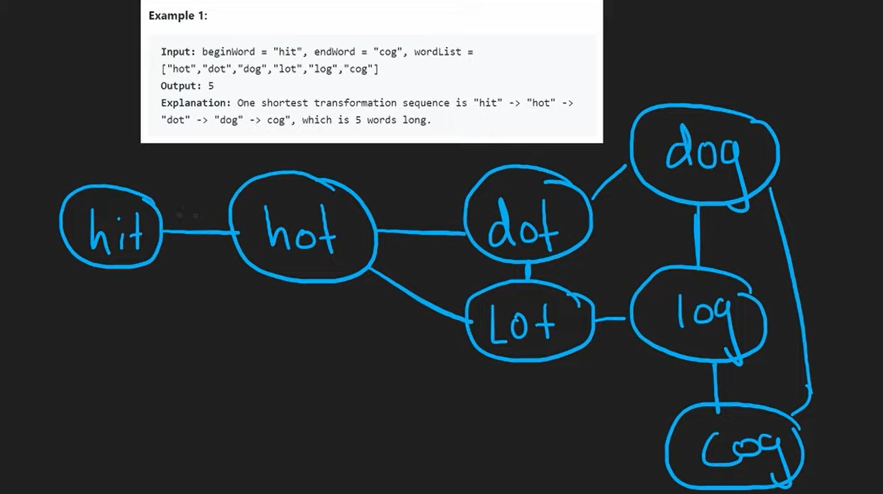
\includegraphics[width=0.4\linewidth,keepaspectratio]{leetwordladder}
\end{center}	

\end{frame}

%%%%%%%%%%%%%%%%%%%%%%%%%%%%%%%%%%%%%%%%%%%%%%%%%%%%%%%%%%%%%%%%%%%%%%
\begin{frame}[fragile]\frametitle{127. Word Ladder (Hard) Not working}


		\begin{lstlisting}[basicstyle=\scriptsize]
def ladderLength(self, beginWord: str, endWord: str, wordList: List[str]) -> int:
    if endWord in wordList:
        return 0

    neighbors = collections.defaultdict(list)
    wordList.append(beginWord)
    for word in wordList:
        for j in range(len(wordList)):
            pattern = word[:j] + "*" + word[j+1:]
            neighbors[pattern].append(word)
    visited = set([beginWord])
    q = collections.deque([beginWord])
    result = 1
    while q:
        for i in range(len(q)):
            word = q.popleft()
            if word == endWord:
                return result
            for j in range(len(word)):
                pattern = word[:j] + "*" + word[j+1:]
                for neighbor_word in neighbors[pattern]:
                    if neighbor_word not in visited:
                        visited.add(neighbor_word)
                        q.append(neighbor_word)
        result += 1
    return 0
				\end{lstlisting}		

	
\end{frame}

%%%%%%%%%%%%%%%%%%%%%%%%%%%%%%%%%%%%%%%%%%%%%%%%%%%%%%%%%%%%%%%%%%%%%%
\begin{frame}[fragile]\frametitle{136. Single Number}

	\begin{columns}[T]
		\column{0.5\linewidth}
	\begin{itemize}
	\item Find single number in list having duplicates. O(n) and no additional space
	\item \lstinline{[2,2,1] => 1}
	\item With extra memory: Build frequency dictionary, but delete entry if frequency is two.
	\item Without extra memory: a bit manipulation (not coded here)
	\end{itemize}
		\column{0.455\linewidth}
		\begin{lstlisting}[basicstyle=\scriptsize]
# with extra memory
def singleNumber_w_memory(nums):
    counts = {}
    for n in nums:
        if n not in counts:
            counts[n] = 1
        else:
            del counts[n]
    return list(counts.keys())[0]
				\end{lstlisting}		

	\end{columns}
		
\end{frame}

%%%%%%%%%%%%%%%%%%%%%%%%%%%%%%%%%%%%%%%%%%%%%%%%%%%%%%%%%%%%%%%%%%%%%%
\begin{frame}[fragile]\frametitle{162. Find Peak Element (Medium)}

	\begin{columns}[T]
		\column{0.455\linewidth}
	\begin{itemize}
	\item A peak element is an element that is strictly greater than its neighbors.
	\item Given an integer array nums, find any peak element, and return its index. 
	\item Example \lstinline|Input: nums = [1,2,3,1]; Output: 2|
	\item Linear search $O(n)$. Even if its not sorted, try binary search and break at the first hit. Becomes $O(\log n)$. How to shift? If triplet is moving up, then shift right. If triplet is moving down, move left. In case of vally, any direction is fine.
	\end{itemize}
		\column{0.455\linewidth}
		\begin{lstlisting}[basicstyle=\scriptsize]
def findPeakElement(self, nums: List[int]) -> int:
    left, right = 0, len(nums) - 1
    while left < right:
        mid = (left + right) // 2
        if nums[mid] < nums[mid + 1]:
            left = mid + 1
        else:
            right = mid
    return left
				\end{lstlisting}		
	\end{columns}
	
	
\end{frame}

%%%%%%%%%%%%%%%%%%%%%%%%%%%%%%%%%%%%%%%%%%%%%%%%%%%%%%%%%%%%%%%%%%%%%%
\begin{frame}[fragile]\frametitle{169. Majority Element}

	\begin{columns}[T]
		\column{0.5\linewidth}
	\begin{itemize}
	\item Find majority element from an array
	\item \lstinline{[3,2,3] => 3}
	\item Build frequency counter dictionary, find max
	\item No need to wait till end, break once you get to half of the length.
	\end{itemize}
		\column{0.455\linewidth}
		\begin{lstlisting}[basicstyle=\scriptsize]
def majorityElement(nums):
    sums = {}
    for n in nums:
        if n not in sums:
            sums[n] = 1
        else:
            sums[n] += 1
        if sums[n] > len(nums) / 2:
            return n

				\end{lstlisting}		

	\end{columns}
		
\end{frame}

%%%%%%%%%%%%%%%%%%%%%%%%%%%%%%%%%%%%%%%%%%%%%%%%%%%%%%%%%%%%%%%%%%%%%%
\begin{frame}[fragile]\frametitle{278. First Bad Version (Easy)}

	\begin{columns}[T]
		\column{0.455\linewidth}
	\begin{itemize}
	\item Suppose you have n versions \lstinline|[1, 2, ..., n]| and you want to find out the first bad one, which causes all the following ones to be bad.
	\item Example 
	\lstinline|Input: n = 5, bad = 4; Output: 4; Explanation: call isBadVersion(3) -> false; call isBadVersion(5) -> true; call isBadVersion(4) -> true; Then 4 is the first bad version.|
	\item Go like Binary Search
	\end{itemize}
		\column{0.455\linewidth}
		\begin{lstlisting}[basicstyle=\scriptsize]
# def isBadVersion(version: int) -> bool:

def firstBadVersion(self, n: int) -> int:
    left, right = 1, n
    while left < right:
        mid = (left + right) // 2
        if isBadVersion(mid):
            right = mid
        else:
            left = mid + 1
    return left
		\end{lstlisting}		
	\end{columns}
	
	
\end{frame}


%%%%%%%%%%%%%%%%%%%%%%%%%%%%%%%%%%%%%%%%%%%%%%%%%%%%%%%%%%%%%%%%%%%%%%
\begin{frame}[fragile]\frametitle{283. Move Zeros}

	\begin{columns}[T]
		\column{0.5\linewidth}
	\begin{itemize}
	\item Given an array, move its zeros to right end, in place
	\item \lstinline{[0,1,2,0,3,12] => [1,2,3,12,0,0]}
	\item Traverse from left, if non zero, see if it can swapped with 0 earlier to stays.
	\item Once done, fill all remaining positions with 0s
	\end{itemize}
		\column{0.455\linewidth}
		\begin{lstlisting}[basicstyle=\scriptsize]
def moveZeros(nums):
    zero_count = nums.count(0)
    next_non_zero = 0
    for n in nums:
        if n != 0:
            nums[next_non_zero] = n
            next_non_zero += 1
    for zero in range(1,zero_count+1):
        nums[-zero] = 0
				\end{lstlisting}		

	\end{columns}
		
\end{frame}

%%%%%%%%%%%%%%%%%%%%%%%%%%%%%%%%%%%%%%%%%%%%%%%%%%%%%%%%%%%%%%%%%%%%%%
\begin{frame}[fragile]\frametitle{374. Guess Number Higher or Lower (Easy)}

	\begin{columns}[T]
		\column{0.455\linewidth}
	\begin{itemize}
	\item I pick a number from 1 to n. You have to guess which number I picked. Every time you guess wrong, I will tell you whether the number I picked is higher or lower than your guess.
	\item Example \lstinline|Input: n = 10, pick = 6;  Output: 6|
	\item Go by binary partitioning.
	\end{itemize}
		\column{0.455\linewidth}
		\begin{lstlisting}[basicstyle=\scriptsize]
def guess(num: int) -> int:
	# has been provided
	
def guessNumber(n):
    left, right = 1, n
    while True:
        mid = (left + right)//2
        user_response = guess(mid)
        if user_response > 0:
            left = mid + 1
        elif user_response < 0 :
            right = mid - 1
        else:
            return mid
				\end{lstlisting}		
	\end{columns}
	
	
\end{frame}
